\begin{frame}{Research Training}
\framesubtitle{LoRaWAN Extension}
\begin{figure}[H]
    \centering
    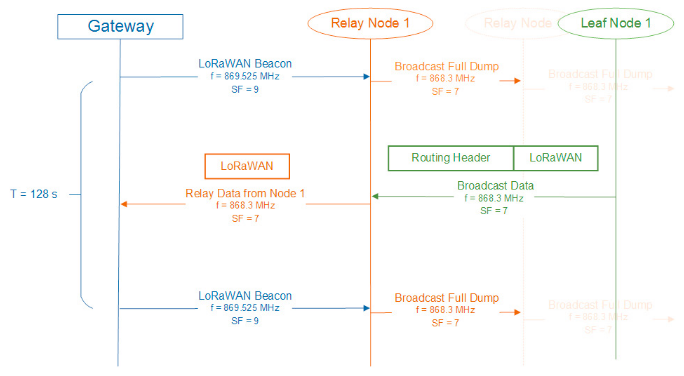
\includegraphics[width=0.98\textwidth]{presentation.tex/fig/lorawanextension.png}
    \caption{LoRaWAN Extension\footnotemark}
\end{figure}

\footcitetext{DIAS2018424}
\end{frame}

\begin{frame}{Research Training}
\framesubtitle{Linear Sensor Network}
\begin{columns}
\begin{column}{0.5\textwidth}
\begin{figure}[H]
    \centering
    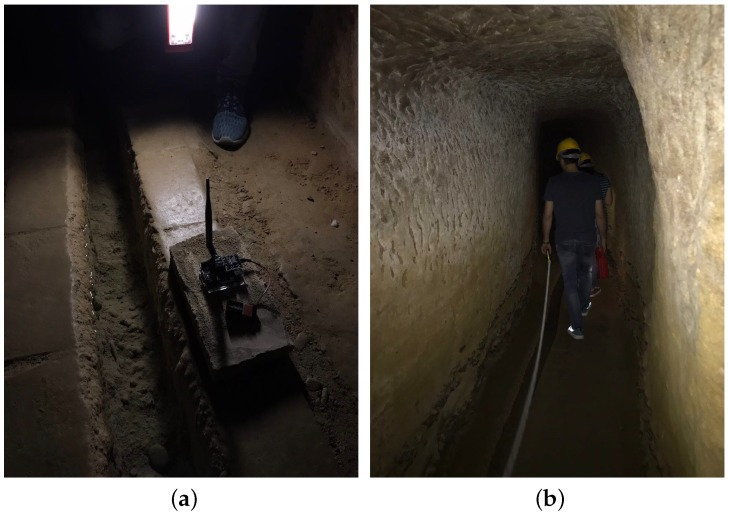
\includegraphics[width=1\textwidth]{presentation.tex/fig/lsnlora.jpg}
    \caption{Underground tunnel installation\footnotemark}
\end{figure}
\end{column}
\begin{column}{0.5\textwidth}
\begin{figure}[H]
    \centering
    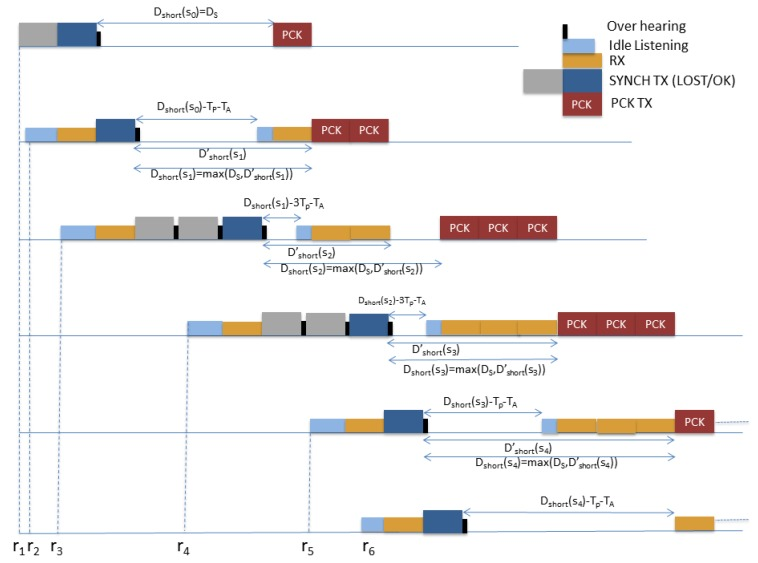
\includegraphics[width=0.98\textwidth]{presentation.tex/fig/lsnlora2.jpg}
    \caption{Protocol\footnotemark}
\end{figure}
\end{column}
\end{columns}
\footcitetext{Abrardo_2019}
\end{frame}

\begin{frame}{Research Training}
\framesubtitle{LoRaBlink}
\begin{columns}
\begin{column}{0.3\textwidth}
\begin{figure}[H]
    \centering
    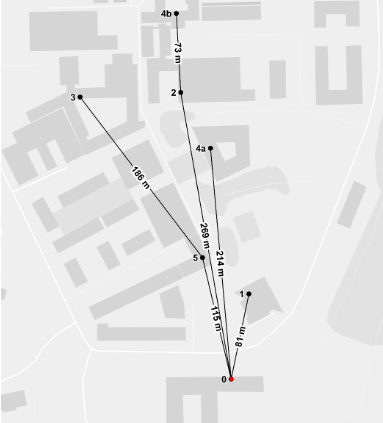
\includegraphics[width=1\textwidth]{presentation.tex/fig/lorablink2.png}
    \caption{Range\footnotemark}
\end{figure}
\end{column}
\begin{column}{0.7\textwidth}
\begin{figure}[H]
    \centering
    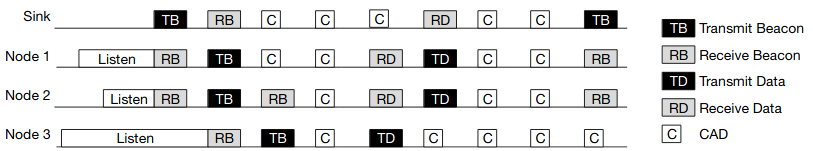
\includegraphics[width=0.98\textwidth]{presentation.tex/fig/lorablink.png}
    \caption{LoRaBlink protocol\footnotemark}
\end{figure}
\end{column}
\end{columns}
\footcitetext{lorablink}
\end{frame}

% \begin{frame}{Research Training}
% \framesubtitle{Solving LoRaWAN issues}
% \begin{figure}[H]
%     \centering
%     \def\angle{0}
%     \def\radius{3}
%     \resizebox{4cm}{4cm}{%
%     \begin{tikzpicture}[nodes = {font=\sffamily}]
%       \foreach \color in {
%             yellow,
%             red,
%             yellow,
%             white,
%             red,
%             yellow,
%             white,
%             yellow,
%             white,
%             white,
%             red,
%             red,
%         } {
%         \ifx\color\empty\else
%             \draw[fill={\color!50},draw={\color}] (0,0) -- (\angle:\radius)
%               arc (\angle:\angle+30:\radius) -- cycle;
%             \pgfmathparse{\angle+30}
%             \xdef\angle{\pgfmathresult}
%         \fi
%         };
%         \xdef\radius{2.5}
%         \foreach \color in {
%             yellow,
%             red,
%             yellow,
%             yellow,
%             red,
%             white,
%             yellow,
%             red,
%             white,
%             white,
%             white,
%             white,
%         } {
%         \ifx\color\empty\else
%             \draw[fill={\color!50},draw={\color}] (0,0) -- (\angle:\radius)
%               arc (\angle:\angle+30:\radius) -- cycle;
%             \pgfmathparse{\angle+30}
%             \xdef\angle{\pgfmathresult}
%         \fi
%         };
%         \xdef\radius{2}
%         \foreach \color in {
%             yellow,
%             red,
%             green,
%             red,
%             yellow,
%             white,
%             yellow,
%             white,
%             white,
%             white,
%             white,
%             white,
%         } {
%         \ifx\color\empty\else
%             \draw[fill={\color!50},draw={\color}] (0,0) -- (\angle:\radius)
%               arc (\angle:\angle+30:\radius) -- cycle;
%             \pgfmathparse{\angle+30}
%             \xdef\angle{\pgfmathresult}
%         \fi
%         };
%         \xdef\radius{1.5}
%         \foreach \color in {
%             yellow,
%             red,
%             yellow,
%             yellow,
%             yellow,
%             green,
%             yellow,
%             white,
%             red,
%             white,
%             white,
%             white,
%         } {
%         \ifx\color\empty\else
%             \draw[fill={\color!50},draw={\color}] (0,0) -- (\angle:\radius)
%               arc (\angle:\angle+30:\radius) -- cycle;
%             \pgfmathparse{\angle+30}
%             \xdef\angle{\pgfmathresult}
%         \fi
%         };
%         \xdef\radius{1}
%         \foreach \color in {
%             green,
%             green,
%             green,
%             yellow,
%             yellow,
%             yellow,
%             white,
%             white,
%             yellow,
%             red,
%             yellow,
%             red,
%         } {
%         \ifx\color\empty\else
%             \draw[fill={\color!50},draw={\color}] (0,0) -- (\angle:\radius)
%               arc (\angle:\angle+30:\radius) -- cycle;
%             \pgfmathparse{\angle+30}
%             \xdef\angle{\pgfmathresult}
%         \fi
%         };
%         \xdef\radius{0.5}
%         \foreach \color in {
%             green,
%             green,
%             yellow,
%             yellow,
%             green,
%             green,
%             yellow,
%             red,
%             yellow,
%             green,
%             green,
%             green,
%         } {
%         \ifx\color\empty\else
%             \draw[fill={\color!50},dotted,draw={\color}] (0,0) -- (\angle:\radius)
%               arc (\angle:\angle+30:\radius) -- cycle;
%             \pgfmathparse{\angle+30}
%             \xdef\angle{\pgfmathresult}
%         \fi
%         };
%         % \path[thick, dotted] (-0.7, -1.1) edge (0,0);
%         % \node[motes] () at (-0.7, -1.1) {};
%         \path[thick, dotted] (-1.5, 2.2) edge (-0.5,1.2);
%         \path[thick, dotted] (0, 0) edge (-0.5,1.2);
%         \node[motes] () at (-1.5, 2.2) {};
%         \node[motes] () at (-0.5, 1.2) {};
%         \path[thick, dotted] (2.5, 2.3) edge (0.5,1.5);
%         \path[thick, dotted] (0.5, 1.3) edge (0,0);
%         \node[motes] () at (2.5, 2.3) {};
%         \node[motes] () at (0.5, 1.3) {};

%         \node[motes] () at (2.2, -2.1) {};
%         \foreach \place/\name in {{(0,0)/a}}
%             \node[gateways] (\name) at \place {};
%     \end{tikzpicture}
%     }
% \end{figure}
% \end{frame}
